%%% linuxessay.tex --- 
%% 
%% Description: Simple Sectioned Essay Template. The \lipsum[#] commands throughout this template generate dummy text to fill the template out. These commands should all be removed when writing essay content.
%% Author: Hongyi Wu(吴鸿毅)
%% Email: wuhongyi@qq.com 
%% Created: 三 9月  9 10:30:38 2015 (+0800)
%% Last-Updated: 四 9月 10 14:06:58 2015 (+0800)
%%           By: Hongyi Wu(吴鸿毅)
%%     Update #: 141
%% URL: http://wuhongyi.github.io 

%----------------------------------------------------------------------------------------
%	PACKAGES AND OTHER DOCUMENT CONFIGURATIONS
%----------------------------------------------------------------------------------------

\documentclass[12pt,a4paper]{article} % Default font size is 12pt, it can be changed here
\usepackage[slantfont,boldfont]{xeCJK} 
\usepackage{geometry} % Required to change the page size to A4
\usepackage{graphicx} % Required for including pictures
\usepackage{lipsum} % Used for inserting dummy 'Lorem ipsum' text into the template
\usepackage{indentfirst}% 首行缩进
\usepackage{setspace}% 调节行间距  
\usepackage{booktabs}% 用于表格中加下划线,cmidrule(r){2-2}
\linespread{1.2} % Line spacing

%\setlength\parindent{0pt} % Uncomment to remove all indentation from paragraphs

\graphicspath{{Pictures/}} % Specifies the directory where pictures are stored

%% \usepackage{times}%让英语默认都是Times New Roman

%% \usepackage[cm-default]{fontspec} %[cm-default]选项主要用来解决使用数学环境时数学符号不能正常显示的问题
\usepackage{fontspec}
\usepackage{xunicode}
\usepackage{xltxtra} 


\XeTeXlinebreaklocale "zh"
\XeTeXlinebreakskip = 0pt plus 1pt minus 0.1pt

%字体重命名,方便使用
%% \newfontfamily\times{Times New Roman}

\newCJKfontfamily{\song}{SimSun}
\newCJKfontfamily{\hei}{SimHei}
\newCJKfontfamily{\kai}{KaiTi}
\newCJKfontfamily{\fangsong}{FangSong}

%系统中文查看命令:fc-list :lang=zh
\setmainfont{Times New Roman}%文档正文默认英语字体,设置衬线字体
%% \setsansfont {}%设定无衬线字体
\setCJKmainfont[BoldFont={SimSun},ItalicFont={KaiTi}]{SimSun}%设置默认中文字体
\setCJKsansfont{SimHei}
\setCJKmonofont{FangSong}% 设置等宽字体
%Sans Serif 无衬线字体 楷体、黑体、幼圆 \sansfont 。Serif 衬线字体 对应中文的 宋、仿宋\mainfont

\newcommand{\yihao}{\fontsize{26pt}{26pt}\selectfont} % 一号, 单倍行距
\newcommand{\erhao}{\fontsize{22pt}{22pt}\selectfont} % 二号, 单倍行距
\newcommand{\xiaoer}{\fontsize{18pt}{18pt}\selectfont} % 小二, 单倍行距
\newcommand{\sanhao}{\fontsize{16pt}{16pt}\selectfont} % 三号, 单倍行距
\newcommand{\xiaosan}{\fontsize{15pt}{15pt}\selectfont} % 小三, 单倍行距
\newcommand{\sihao}{\fontsize{14pt}{14pt}\selectfont} % 四号, 单倍行距
\newcommand{\banxiaosi}{\fontsize{13pt}{13pt}\selectfont} % 半小四, 单倍行距
\newcommand{\xiaosi}{\fontsize{12pt}{12pt}\selectfont} % 小四, 单倍行距
\newcommand{\dawuhao}{\fontsize{11.5pt}{11.5pt}\selectfont} % 大五号, 单倍行距
\newcommand{\wuhao}{\fontsize{10.5pt}{10.5pt}\selectfont} % 五号, 单倍行距
\newcommand{\xiaowu}{\fontsize{9.5pt}{9.5pt}\selectfont} % 小五号, 单倍行距
\newcommand{\banbanxiaosi}{\fontsize{12pt}{12pt}\selectfont}% 半半小四, 单倍行距
\defaultfontfeatures{Mapping=tex-text}%如果没有它会有一些tex特殊字符无法正常使用,比如连字符
\XeTeXdefaultencoding"UTF8"

\begin{document}

%----------------------------------------------------------------------------------------
%	TITLE PAGE
%----------------------------------------------------------------------------------------

\begin{titlepage}

\newcommand{\HRule}{\rule{\linewidth}{0.5mm}} % Defines a new command for the horizontal lines, change thickness here

\center % Center everything on the page

\textsc{\LARGE Peking University }\\[1.5cm] % Name of your university/college
\textsc{\Large Major Heading}\\[0.5cm] % Major heading such as course name
\textsc{\large Minor Heading}\\[0.5cm] % Minor heading such as course title

\HRule \\[0.4cm]
{ \huge \bfseries Title}\\[0.4cm] % Title of your document
\HRule \\[1.5cm]

\begin{minipage}{0.4\textwidth}
\begin{flushleft} \large
\emph{Author:}\\
Hongyi Wu %John \textsc{Smith} % Your name
\end{flushleft}
\end{minipage}
~
\begin{minipage}{0.4\textwidth}
\begin{flushright} \large
\emph{Supervisor:} \\
XX X  %Dr. James \textsc{Smith} % Supervisor's Name
\end{flushright}
\end{minipage}\\[4cm]

{\large \today}\\[3cm] % Date, change the \today to a set date if you want to be precise


\includegraphics{logo.jpeg}\\[1cm] % Include a department/university logo - this will require the graphicx package

\vfill % Fill the rest of the page with whitespace

\end{titlepage}

%----------------------------------------------------------------------------------------
%	TABLE OF CONTENTS
%----------------------------------------------------------------------------------------

\tableofcontents % Include a table of contents

\newpage % Begins the essay on a new page instead of on the same page as the table of contents 

%----------------------------------------------------------------------------------------
%	INTRODUCTION
%----------------------------------------------------------------------------------------

\section{Introduction} % Major section

这里是开始。 Example citation \cite{Figueredo:2009dg}.

%------------------------------------------------

\subsection{Subsection 1} % Sub-section

\lipsum[1] % Dummy text

%------------------------------------------------

\subsection{Subsection 2} % Sub-section

\lipsum[2] % Dummy text

%------------------------------------------------

\subsubsection{Subsubsection 1} % Sub-sub-section

\lipsum[3] % Dummy text

\begin{figure}[h] % Example image
\center{
\includegraphics[width=0.5\linewidth]{placeholder.png}}
\caption{Example image.}
\label{fig:speciation}
\end{figure}

%------------------------------------------------

\subsubsection{Subsubsection 2} % Sub-sub-section

\lipsum[4] % Dummy text

%----------------------------------------------------------------------------------------
%	MAJOR SECTION 1
%----------------------------------------------------------------------------------------

\section{Content Section} % Major section

\lipsum[5] % Dummy text

%------------------------------------------------

\subsection{Subsection 1} % Sub-section

\subsubsection{Subsubsection 1} % Sub-sub-section

\lipsum[6] % Dummy text

%------------------------------------------------

\subsubsection{Subsubsection 2} % Sub-sub-section

\lipsum[6] % Dummy text
\begin{figure}[!htb]
  \begin{center}
    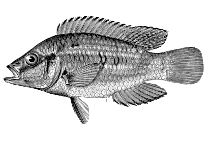
\includegraphics[width=0.38\textwidth]{fish.png}
  \end{center}
  \caption{Fish}
\end{figure}
\lipsum[7-8] % Dummy text

%------------------------------------------------

\subsubsection{Subsubsection 3} % Sub-sub-section

\begin{description} % Numbered list example

\item[第一] \hfill \\
\lipsum[9] % Dummy text

\item[Second] \hfill \\
\lipsum[10] % Dummy text

\item[Third] \hfill \\
\lipsum[11] % Dummy text

\end{description} 

%----------------------------------------------------------------------------------------
%	MAJOR SECTION X - TEMPLATE - UNCOMMENT AND FILL IN
%----------------------------------------------------------------------------------------

\section{\song{中文标题测试}}

\subsection{\song{测试} 1} % Sub-section

{\kai 这里是正文测试。这里是正文测试。这里是正文测试。这里是正文测试。这里是正文测试}{\hei abcdesghijklmnopqrstuvwxyz} 这里是正文测试。这里是正文测试。这里是正文测试。这里是正文测试。这里是正文测试。这里是正文测试。

{\kai 这里是正文测试。这里是正文测试。这里是正文测试。这里是正文测试。这里是正文测试。}

%------------------------------------------------

\subsection{\song{测试} 2} % Sub-section

这里是正文测试。这里是正文测试。这里是正文测试。这里是正文测试。这里是正文测试。这里是正文测试。

{\hei 这里是正文测试。这里是正文测试。这里是正文测试。这里是正文测试。这里是正文测试。}这里是正文测试。这里是正文测试。这里是正文测试。这里是正文测试。这里是正文测试。这里是正文测试。这里是正文测试。

%----------------------------------------------------------------------------------------
%	CONCLUSION
%----------------------------------------------------------------------------------------

\section{Conclusion} % Major section

%\lipsum[12-13]
There is a test about fonts of xaletex.

这里是正文测试。这里是正文测试。这里是正文测试。
$a^2+b^2=c^2$
%----------------------------------------------------------------------------------------
%	BIBLIOGRAPHY
%----------------------------------------------------------------------------------------

%% \begin{thebibliography}{99} % Bibliography - this is intentionally simple in this template
%% \bibitem[Figueredo and Wolf, 2009]{Figueredo:2009dg}
%% Figueredo, A.~J. and Wolf, P. S.~A. (2009).
%% \newblock Assortative pairing and life history strategy - a cross-cultural
%%   study.
%% \newblock {\em Human Nature}, 20:317--330.
%% \end{thebibliography}

\bibliographystyle{unsrt}
\bibliography{reference}

%----------------------------------------------------------------------------------------

\end{document}

%%%%%%%%%%%%%%%%%%%%%%%%%%%%%%%%%%%%%%%%%%%%%%%%%%%%%%%%%%%%%%%%%%%%%%
%%% linuxessay.tex ends here
